Wanneer gekeken wordt naar figuur \ref{fig:tijd} valt meteen op dat \textit{Fast Non-Local Mean Denoising} voor om het even welke kern grootte niet echt efficiënt is. Dit kon alreeds verwacht worden door de manier waarop deze methode te werk gaat. De waarde blijft nagenoeg constant geacht de kern grootte maar is trager met een orde van grootte 3 ten opzichte van de andere filters. Om deze reden zal deze filter al zeker niet opgenomen worden in het project. 

\begin{figure}[h!]
    \centering
    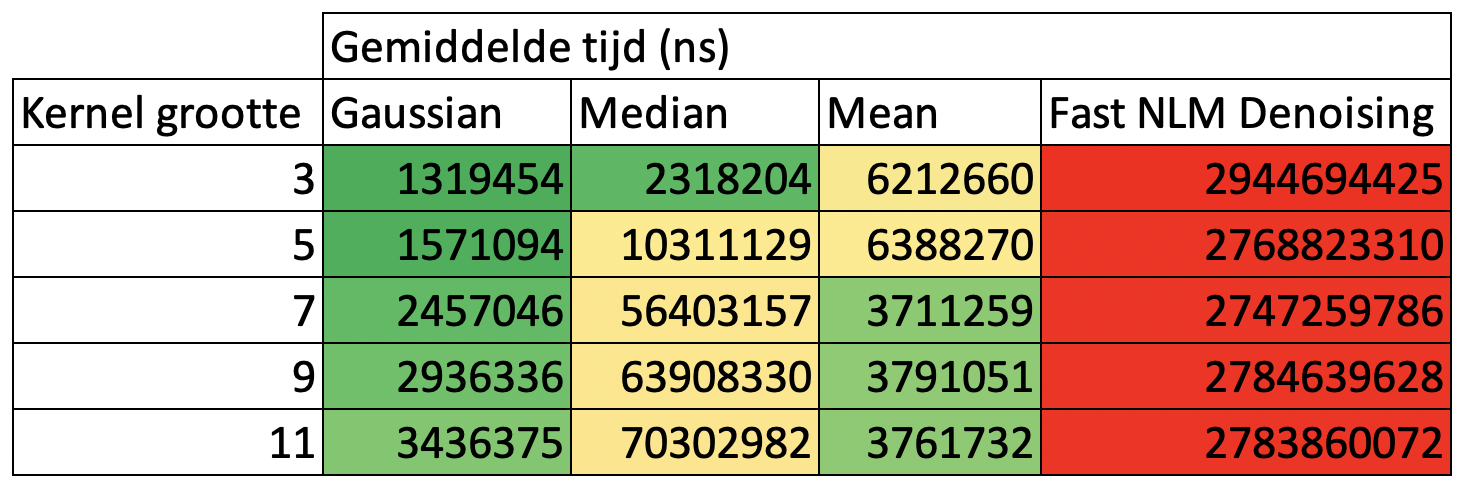
\includegraphics[scale=0.5]{img/tijdsconsumptie}
    \caption{Gemiddelde tijd nodig om filter op afbeelding toe te passen.}
    \label{fig:tijd}
\end{figure}

Voor de andere filters kunnen hun individuele tijdsgrafieken \ref{fig:tijdsgrafieken} van dichterbij bekeken worden. 
Bij de \textit{Gaussian filter} is een duidelijk lineair verband tussen kerngrootte en tijdsconsumptie zichtbaar. Dit wordt bevestigd door de determinatiecoëfficiënt van 97,85 procent van de lineaire trendlijn. 


Verder zijn er nog twee opvallende zaken. Enerzijds zorgt een grotere kern ervoor dat de \textit{Median filter} veel meer tijd nodig heeft. De reden hiervoor is dat hoe groter de kern, hoe meer elementen pixelwaarden gesorteerd moeten worden van van klein naar groot.

Bij de \textit{Mean filter} houden de waarden er nagenoeg constante waarde. Rond kern grootte 6 gebeurt een sprong in uitvoeringstijd. 
WHY??????????????????????????

 \begin{figure}[h!]
  \centering
  \begin{subfigure}{0.4\linewidth}
    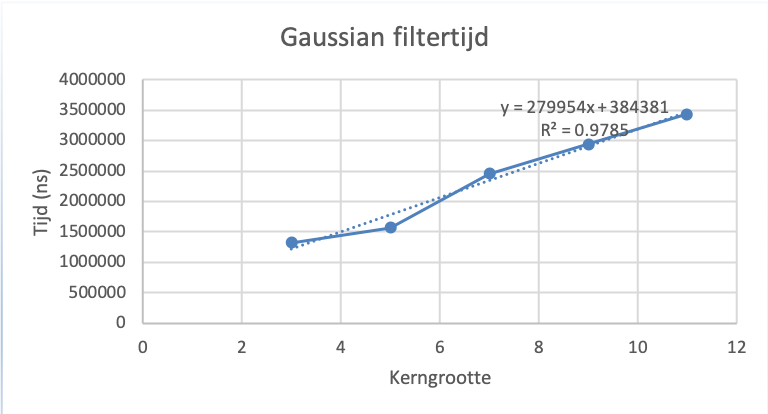
\includegraphics[width=\linewidth]{img/gaussiantijd}
  \end{subfigure}
  \begin{subfigure}{0.4\linewidth}
    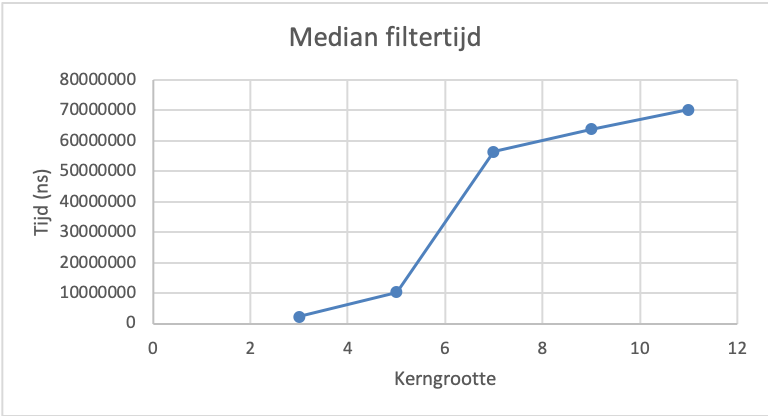
\includegraphics[width=\linewidth]{img/mediantijd}
  \end{subfigure}
  \begin{subfigure}{0.4\linewidth}
    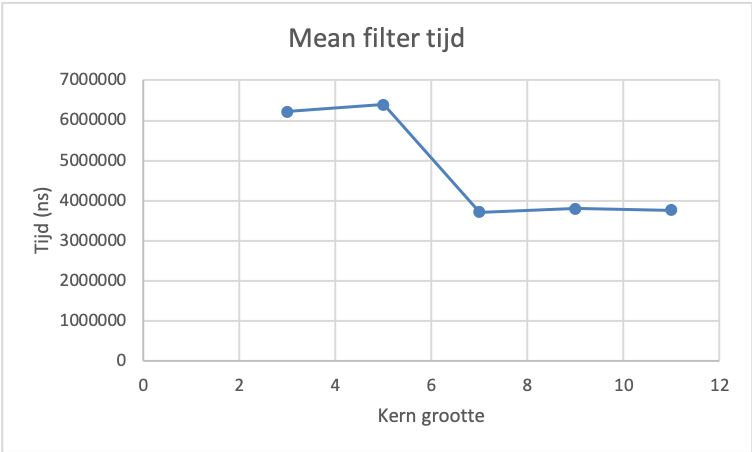
\includegraphics[width=\linewidth]{img/meantijd}
  \end{subfigure}
  \caption{Tijdsgrafieken voor de verschillende filters}
  \label{fig:tijdsgrafieken}
\end{figure}

Wanneer naar de tijdscomponent gekeken wordt geven \textit{Gaussian en Median filter} de beste resultaten. 
Op basis van tijd wordt de laatste methode al afgeschreven. 



